\documentclass{article}

\usepackage[final]{neurips_2023}

\usepackage[utf8]{inputenc}
\usepackage[T1]{fontenc}
\usepackage{hyperref}
\usepackage{url}
\usepackage{booktabs}
\usepackage{amsfonts}
\usepackage{nicefrac}
\usepackage{microtype}
\usepackage{xcolor}
\usepackage{graphicx}
\usepackage{float}
\usepackage{subfigure}
\usepackage{amsmath}


\title{Why Detectors Fail on Unseen Generators:\\
Ablation, Feature-Space Analysis, and a Route Towards Mixture-of-Experts Detection}


\author{
  Anonymous Author
}


\begin{document}

\maketitle


\begin{abstract}
The rapid advancement of generative models—spanning GANs, diffusion models, and autoregressive architectures—has made AI-generated image detection an increasingly critical task for forensics and content moderation.
Existing detectors often achieve high accuracy on known generators but fail to generalise to unseen ones.
In this paper, we conduct a systematic ablation study on the GenImage benchmark, comparing five detection strategies across four generators: GLIDE (in-distribution), BigGAN, ADM, and VQDM.
We evaluate full fine-tuning and linear probing on ResNet-18, ViT-Small, and CLIP-ViT backbones, as well as a cosine-similarity KNN classifier following Ojha~et~al.~\cite{ojha2023towards}.
Our results show that full fine-tuning dominates on in-distribution and GAN-type generators (up to 99.3\%), but all methods collapse to near-chance performance on diffusion-based generators from different families (ADM: 54--65\%, VQDM: 52--65\%).
Notably, CLIP-ViT KNN achieves the best cross-generator accuracy on the hardest generators, supporting the hypothesis that frozen vision-language features generalise better than task-specific features.
We further analyse patch-level classification consistency and discuss a mixture-of-experts framework as a promising direction for truly universal detection.
\end{abstract}


\section{Introduction}

The proliferation of generative AI systems has dramatically lowered the barrier to producing photorealistic synthetic images.
GANs~\cite{goodfellow2014gan}, diffusion models~\cite{dhariwal2021diffusion, rombach2022latent}, and autoregressive generators can now produce images indistinguishable from photographs by the human eye.
This creates urgent demand for robust automatic detectors that can flag AI-generated content for forensics, misinformation prevention, and content moderation.

A natural starting point is to train a binary classifier to distinguish real photographs from AI-generated images.
Simple approaches based on CNN feature extractors achieve near-perfect accuracy within a known generator~\cite{wang2020cnn}.
However, the core challenge is \emph{cross-generator generalisation}: a detector trained on one generator's outputs typically fails when tested on a different generator, because each model leaves distinct low-level artifacts in pixel space~\cite{ojha2023towards}.

Two broad strategies have emerged to address this.
The first is \emph{data diversity}: training on images from many generators so the model learns generator-agnostic cues~\cite{zhu2023genimage}.
The second is \emph{representation universality}: replacing task-specific feature learning with frozen representations from large pretrained models, notably CLIP, which encode broad visual statistics without overfitting to specific generator artifacts~\cite{ojha2023towards}.
A complementary direction exploits physical properties of the generation process itself: DIRE~\cite{wang2023dire} measures the reconstruction error when a diffusion model is used to re-synthesise an image, exploiting the observation that real images are harder to reconstruct than generated ones.

Despite these advances, no single method generalises robustly across all generator families.
This paper investigates \emph{why} through a controlled ablation study on a curated GenImage subset, and provides empirical evidence on the relative strengths of different backbone and training-strategy combinations.

Our main contributions are:
\begin{itemize}
    \item A systematic comparison of five detection strategies (full fine-tuning and linear probing on ResNet-18, ViT-Small, CLIP-ViT; and CLIP KNN) across four generators spanning two distinct generator families.
    \item Quantitative evidence that all current methods fail to generalise from GAN-style generators to diffusion-model generators, with accuracy near chance on ADM and VQDM.
    \item An analysis of patch-level classification consistency revealing that detector errors are spatially systematic rather than localised.
    \item A discussion of a mixture-of-experts (MoE) architecture as a principled future direction for universal detection.
    \item Empirical evidence, via unsupervised clustering of fine-tuned ViT-Small features, that task supervision implicitly organises the feature space by generator family—directly supporting the feasibility of MoE routing.
\end{itemize}


\section{Related Work}

\paragraph{CNN-based fake image detection.}
Wang~et~al.~\cite{wang2020cnn} demonstrated that a ResNet-50 trained on ProGAN images can generalise to some unseen GANs, but fails on diffusion and autoregressive generators.
The key insight is that CNNs learn low-level frequency artifacts (e.g., spectral peaks at regular intervals) specific to a given generator.

\paragraph{Universal detectors.}
Ojha~et~al.~\cite{ojha2023towards} proposed using frozen CLIP features with a linear probe or nearest-neighbour classifier.
By leveraging the broad visual representations learned from 400 million image-text pairs, their approach avoids overfitting to generator-specific fingerprints and achieves strong generalisation, improving over the state of the art by +15 mAP and +25\% accuracy on unseen generators.

\paragraph{Diffusion-specific detection.}
DIRE~\cite{wang2023dire} exploits the generative process directly: an image is re-synthesised by a diffusion model, and the pixel-space reconstruction error is used as a detection signal.
Real images incur high reconstruction error because the diffusion model is not trained on them, while diffusion-generated images are nearly perfectly reconstructed.
This approach is particularly effective for detecting diffusion-model outputs but less effective for GAN-generated images.

\paragraph{Large-scale benchmarks.}
GenImage~\cite{zhu2023genimage} provides over one million real-fake image pairs from eight generators, establishing a standard benchmark for cross-generator generalisation.
We construct a balanced subset of this benchmark for our experiments.


\section{Method}

\subsection{Dataset and Experimental Setup}

We construct a subset of the GenImage benchmark~\cite{zhu2023genimage} from the \texttt{shimei123/Genimage} repository on HuggingFace.
We select four generators covering two distinct architectural families:

\begin{itemize}
    \item \textbf{GLIDE} (diffusion, text-conditioned): used as the \emph{training} source. Train: 4\,000 real + 4\,000 fake; Val: 1\,000 + 1\,000.
    \item \textbf{BigGAN} (GAN, class-conditioned): cross-generator test set, 500 real + 500 fake.
    \item \textbf{ADM} (diffusion, class-conditioned): cross-generator test set, 500 + 500.
    \item \textbf{VQDM} (vector-quantised diffusion): cross-generator test set, 500 + 500.
\end{itemize}

All images are resized and centre-cropped to $224 \times 224$.
Standard ImageNet normalisation is applied for ResNet-18 and ViT-Small; CLIPImageProcessor preprocessing is used for CLIP-ViT.

\subsection{Backbone Architectures}

We evaluate three backbone architectures:

\paragraph{ResNet-18~\cite{he2016deep}.}
An 11M-parameter residual CNN pretrained on ImageNet-1K.
The final fully-connected layer is replaced with a binary classification head.

\paragraph{ViT-Small (patch16/224).}
A 22M-parameter Vision Transformer~\cite{dosovitskiy2021vit} pretrained on ImageNet-21K via the \texttt{timm} library.
The classification token embedding is fed to a linear head.

\paragraph{CLIP-ViT-B/32~\cite{radford2021clip}.}
An 86M-parameter Vision Transformer trained with contrastive language-image supervision on 400M web-crawled image-text pairs.
The pooled vision encoder output is fed to a linear head.

\subsection{Training Strategies}

For each backbone we evaluate two training strategies:

\paragraph{Full Fine-tuning (Full FT).}
All backbone parameters and the classification head are jointly optimised with AdamW (lr=$10^{-4}$, weight decay=$10^{-4}$, 30 epochs, batch size 64).
A ReduceLROnPlateau scheduler (patience=3, factor=0.5) is used.
Data augmentation: random resized crop (scale 0.8--1.0) and horizontal flip.

\paragraph{Linear Probe (LP).}
The backbone is frozen; only the linear classification head is optimised with AdamW (lr=$10^{-3}$, same schedule).
This tests whether pretrained representations alone are sufficient for detection without task-specific adaptation.

\paragraph{CLIP-ViT KNN.}
Following Ojha~et~al.~\cite{ojha2023towards}, the CLIP-ViT backbone is kept frozen.
L2-normalised feature embeddings of all training images are stored as a memory bank.
Test samples are classified by cosine-similarity $k$-nearest-neighbour voting ($k=1$).
No gradient update is performed.

\subsection{Patch-Level Analysis}

To probe whether detection signals are spatially localised, we divide each test image into a $3 \times 3$ grid of non-overlapping patches, classify each patch independently using the ResNet-18 Full FT model, and aggregate predictions by majority vote.
We report both the majority-vote accuracy and the \emph{mean patch consistency}: the fraction of the nine patches that agree with the final voted prediction.


\section{Experiments}

\subsection{Main Results}

Table~\ref{tab:main} reports accuracy on all four test sets.
Figure~\ref{fig:comparison} visualises the full comparison.

\begin{table}[H]
\centering
\caption{Detection accuracy (\%) across methods and generators. All models trained exclusively on GLIDE. \textbf{Bold}: best per column. GLIDE is in-distribution; BigGAN, ADM, VQDM are zero-shot cross-generator tests.}
\label{tab:main}
\begin{tabular}{llcccc}
\toprule
\textbf{Backbone} & \textbf{Strategy} & \textbf{GLIDE} & \textbf{BigGAN} & \textbf{ADM} & \textbf{VQDM} \\
\midrule
ResNet-18  & Full FT       & 98.2          & \textbf{99.3}  & 56.2          & 53.0          \\
ViT-Small  & Full FT       & \textbf{98.7} & 97.8           & 54.9          & 52.1          \\
ResNet-18  & Linear Probe  & 92.0          & 91.9           & 59.4          & 54.7          \\
CLIP-ViT   & Linear Probe  & 99.3          & 98.3           & 61.3          & 55.6          \\
CLIP-ViT   & KNN ($k$=1)   & 85.4          & 81.7           & \textbf{64.9} & \textbf{64.7} \\
\midrule
ResNet-18  & Patch Vote (3$\times$3) & 61.5 & 54.0 & 60.8 & 61.8 \\
\bottomrule
\end{tabular}
\end{table}

\begin{figure}[H]
    \centering
    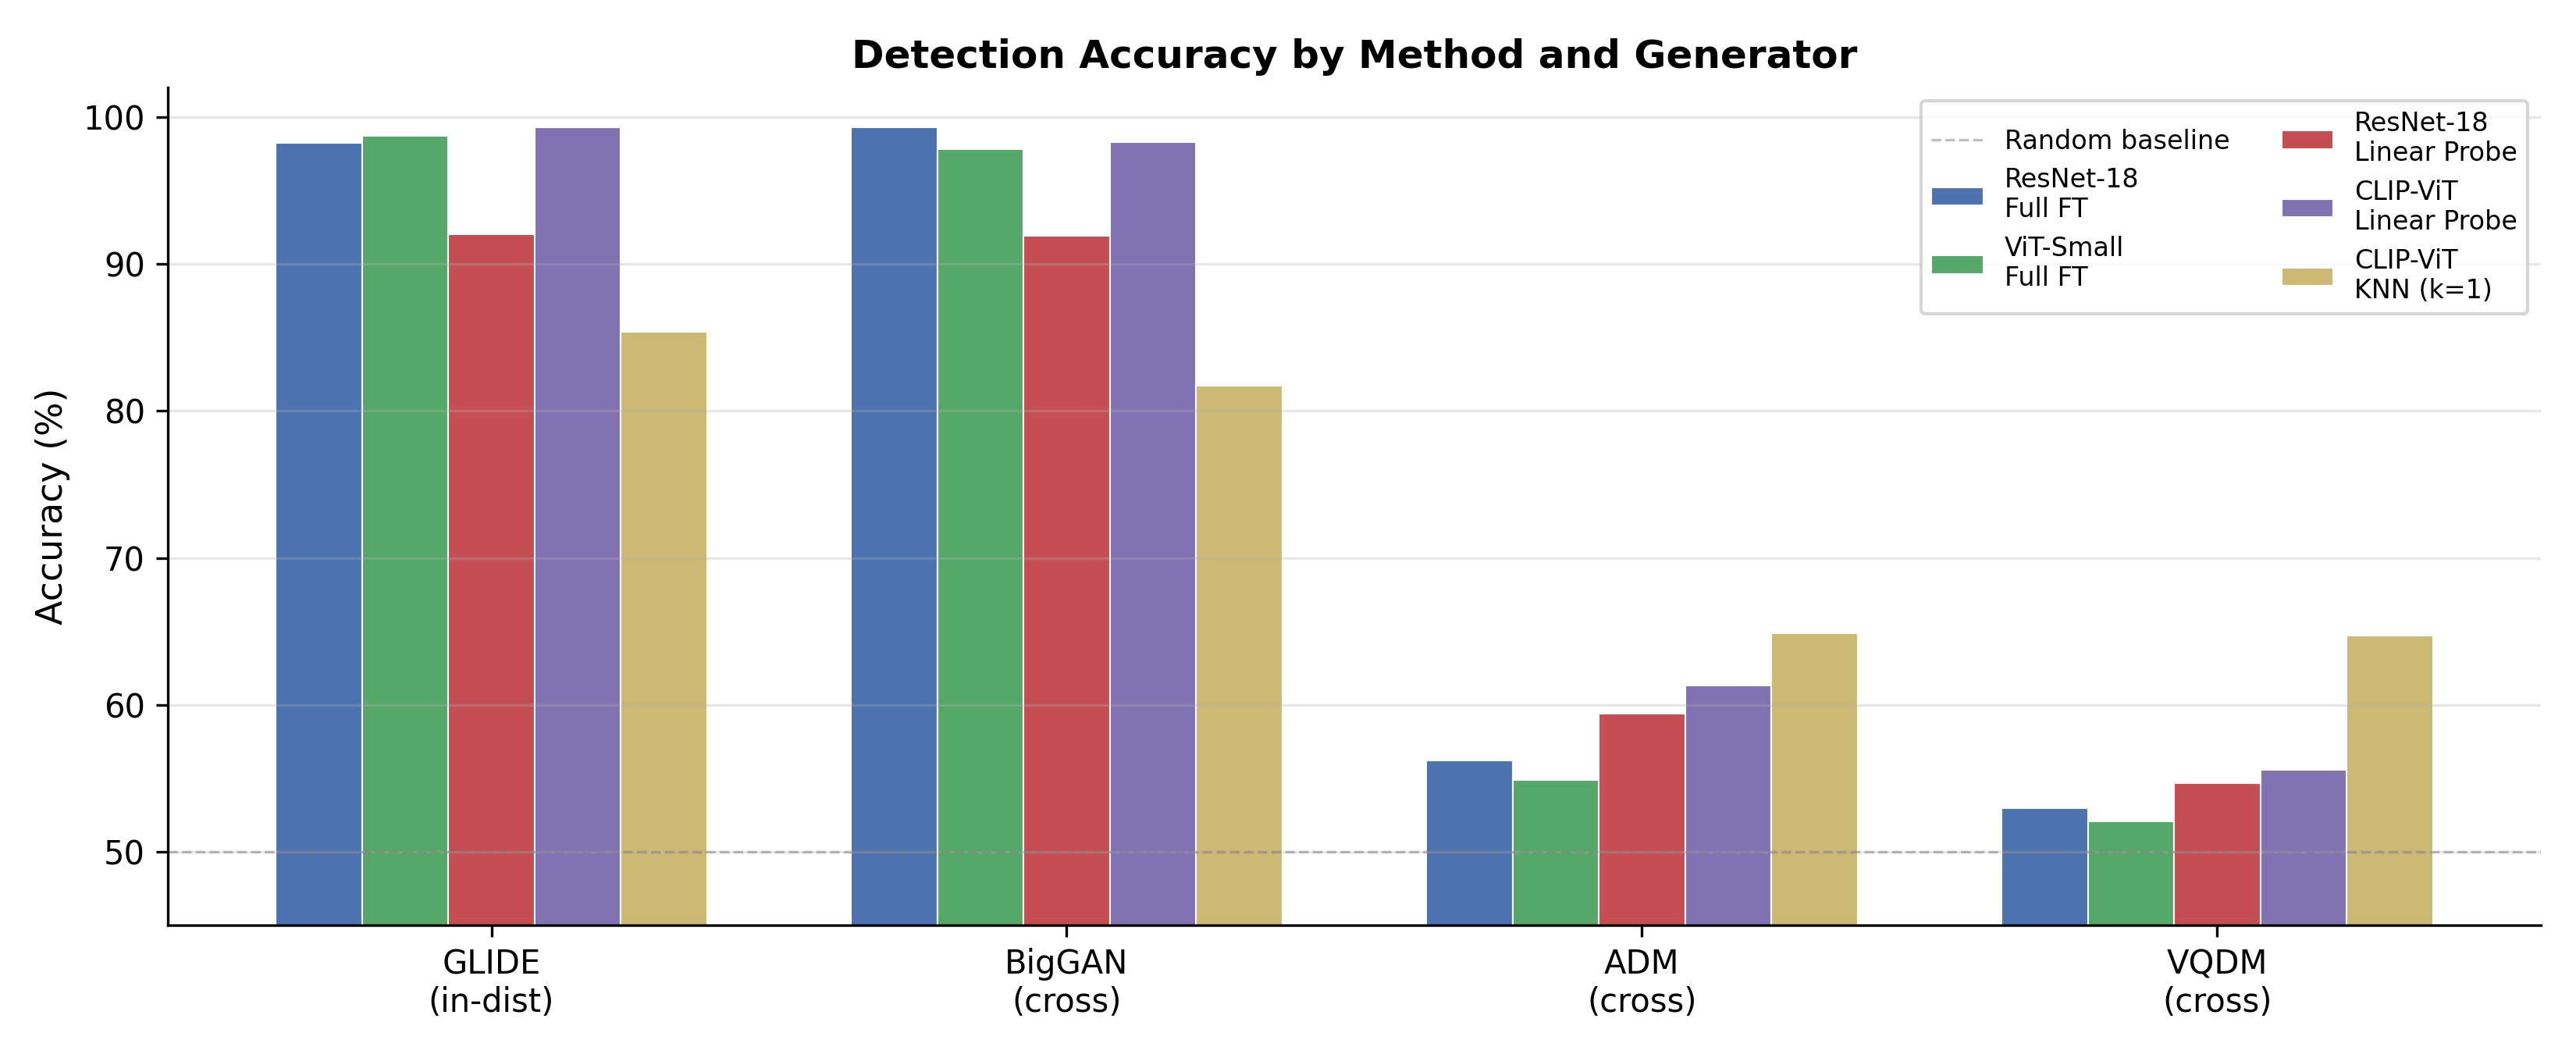
\includegraphics[width=\textwidth]{fig1_accuracy_comparison.png}
    \caption{Detection accuracy by method and generator. All models trained on GLIDE only. Dashed line indicates random-chance baseline (50\%).}
    \label{fig:comparison}
\end{figure}

\subsection{Training Dynamics}

Figure~\ref{fig:curves} shows the training and validation loss/accuracy curves for the ResNet-18 Full FT baseline.
Training loss converges to near zero by epoch 5, while validation accuracy plateaus around 98.5\% from epoch 9, with the best checkpoint at epoch 23 (98.55\%).
The gap between training accuracy ($\approx$100\%) and validation accuracy ($\approx$98.5\%) indicates mild overfitting, though validation performance remains stable throughout training.

\begin{figure}[H]
    \centering
    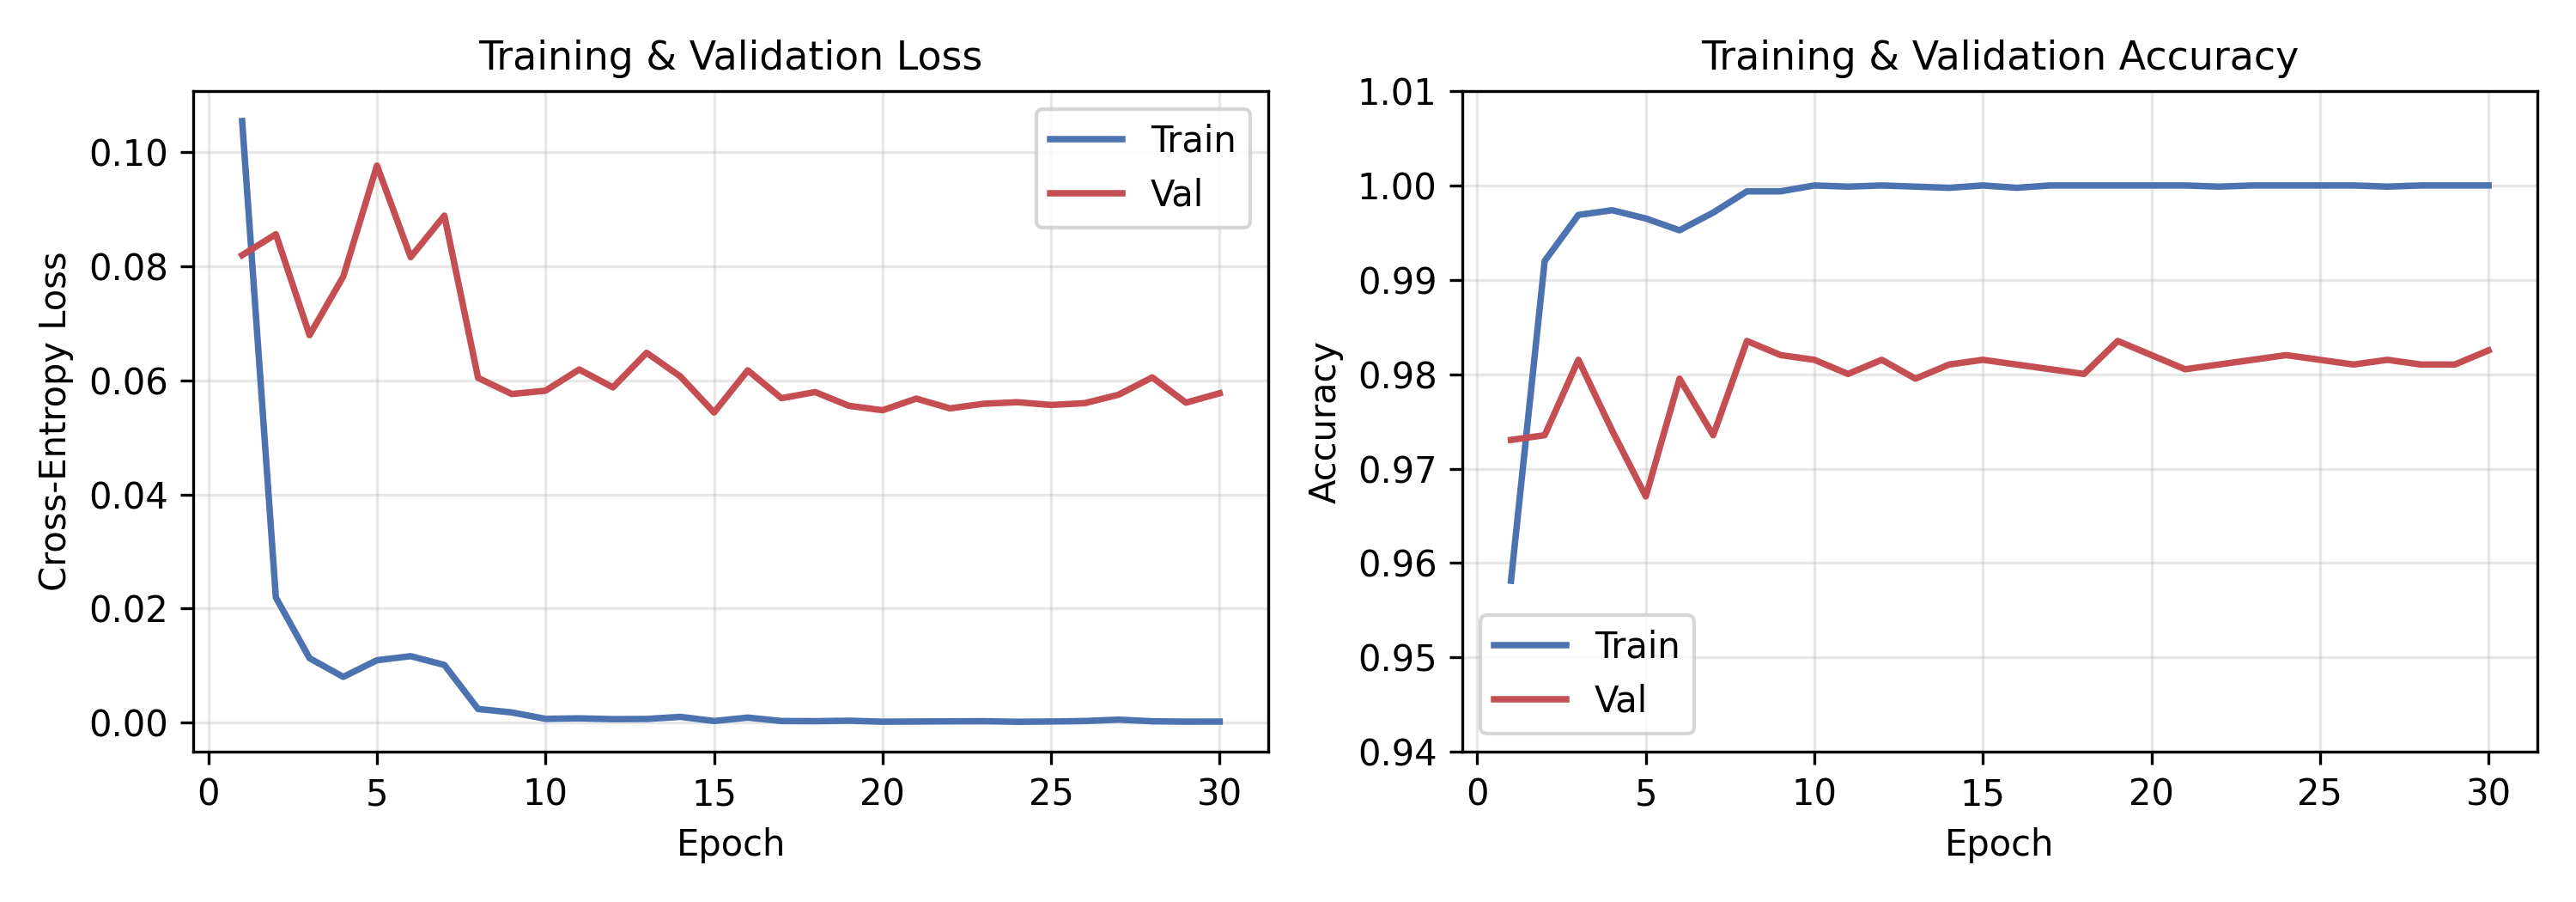
\includegraphics[width=\textwidth]{fig2_training_curves.png}
    \caption{Training and validation loss and accuracy for ResNet-18 Full FT over 30 epochs.}
    \label{fig:curves}
\end{figure}

\subsection{Backbone and Strategy Ablation}

\paragraph{Full fine-tuning vs.\ linear probe.}
Full FT consistently outperforms LP on in-distribution data (ResNet-18: 98.2\% vs.\ 92.0\%; CLIP-ViT: not directly comparable as full FT was not evaluated for CLIP due to computational constraints).
This confirms that end-to-end feature adaptation learns task-specific cues absent from frozen pretrained representations.

\paragraph{Backbone comparison on in-distribution.}
All three backbones achieve high accuracy on GLIDE: ResNet-18 FT (98.2\%), ViT-Small FT (98.7\%), CLIP-ViT LP (99.3\%).
The differences are small, suggesting that the in-distribution task is sufficiently easy for any modern backbone.

\paragraph{Cross-generator generalisation.}
The more revealing comparison is on unseen generators (Figure~\ref{fig:crossgen}).
On BigGAN, full fine-tuning methods remain strong (97.8--99.3\%), because BigGAN and GLIDE share ImageNet-aligned content statistics.
On ADM and VQDM, all fine-tuned models collapse to 52--61\%, barely above chance.
The CLIP-ViT KNN method achieves the highest cross-generator accuracy on ADM (64.9\%) and VQDM (64.7\%), aligning with the findings of Ojha~et~al.~\cite{ojha2023towards} that frozen vision-language features generalise better.

\begin{figure}[H]
    \centering
    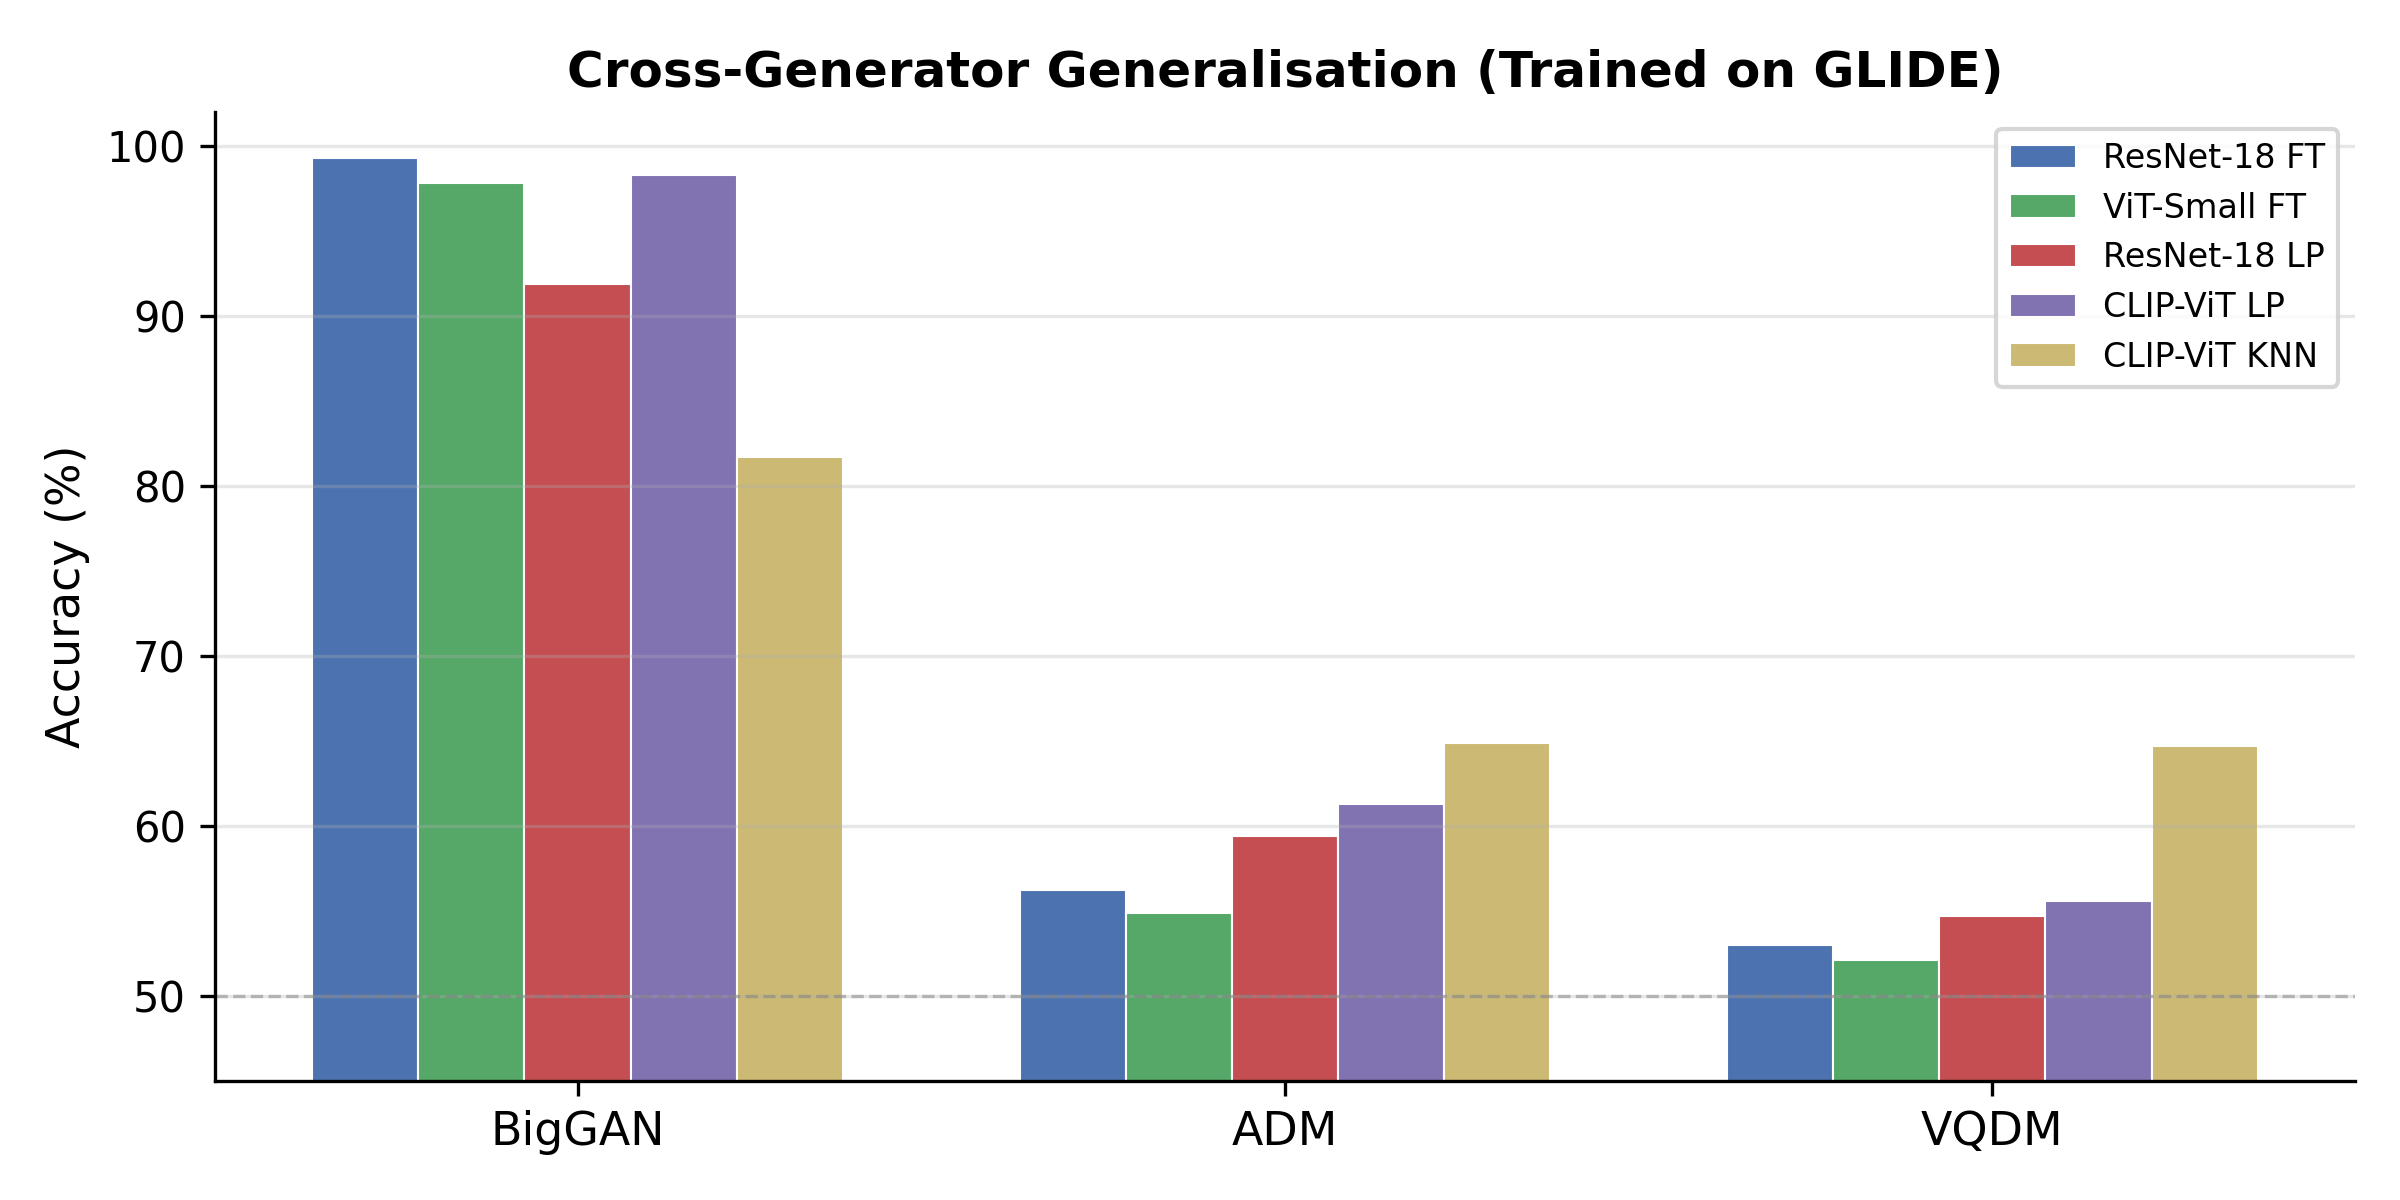
\includegraphics[width=\textwidth]{fig3_cross_gen.png}
    \caption{Cross-generator generalisation on BigGAN, ADM, and VQDM (all zero-shot). Models trained on GLIDE only.}
    \label{fig:crossgen}
\end{figure}

\subsection{Patch-Level Consistency Analysis}

Table~\ref{tab:patch} and Figure~\ref{fig:patch} report patch-level results.
Despite low majority-vote accuracy (54--62\%), patch predictions are highly consistent across spatial locations (87--92\% agreement).
This indicates that when the model is wrong, it tends to be \emph{uniformly} wrong across all patches, rather than making localised errors.
The finding suggests that detection failures are driven by global feature distribution mismatch rather than spatially localised artifacts—a critical insight for future detector design.

\begin{table}[H]
\centering
\caption{Patch-level majority-vote accuracy and mean patch consistency for ResNet-18 Full FT with $3 \times 3$ grid.}
\label{tab:patch}
\begin{tabular}{lcc}
\toprule
\textbf{Generator} & \textbf{Accuracy (\%)} & \textbf{Mean Consistency (\%)} \\
\midrule
GLIDE (in-dist) & 61.5 & 92.4 \\
BigGAN          & 54.0 & 86.5 \\
ADM             & 60.8 & 89.6 \\
VQDM            & 61.8 & 89.6 \\
\bottomrule
\end{tabular}
\end{table}

\begin{figure}[H]
    \centering
    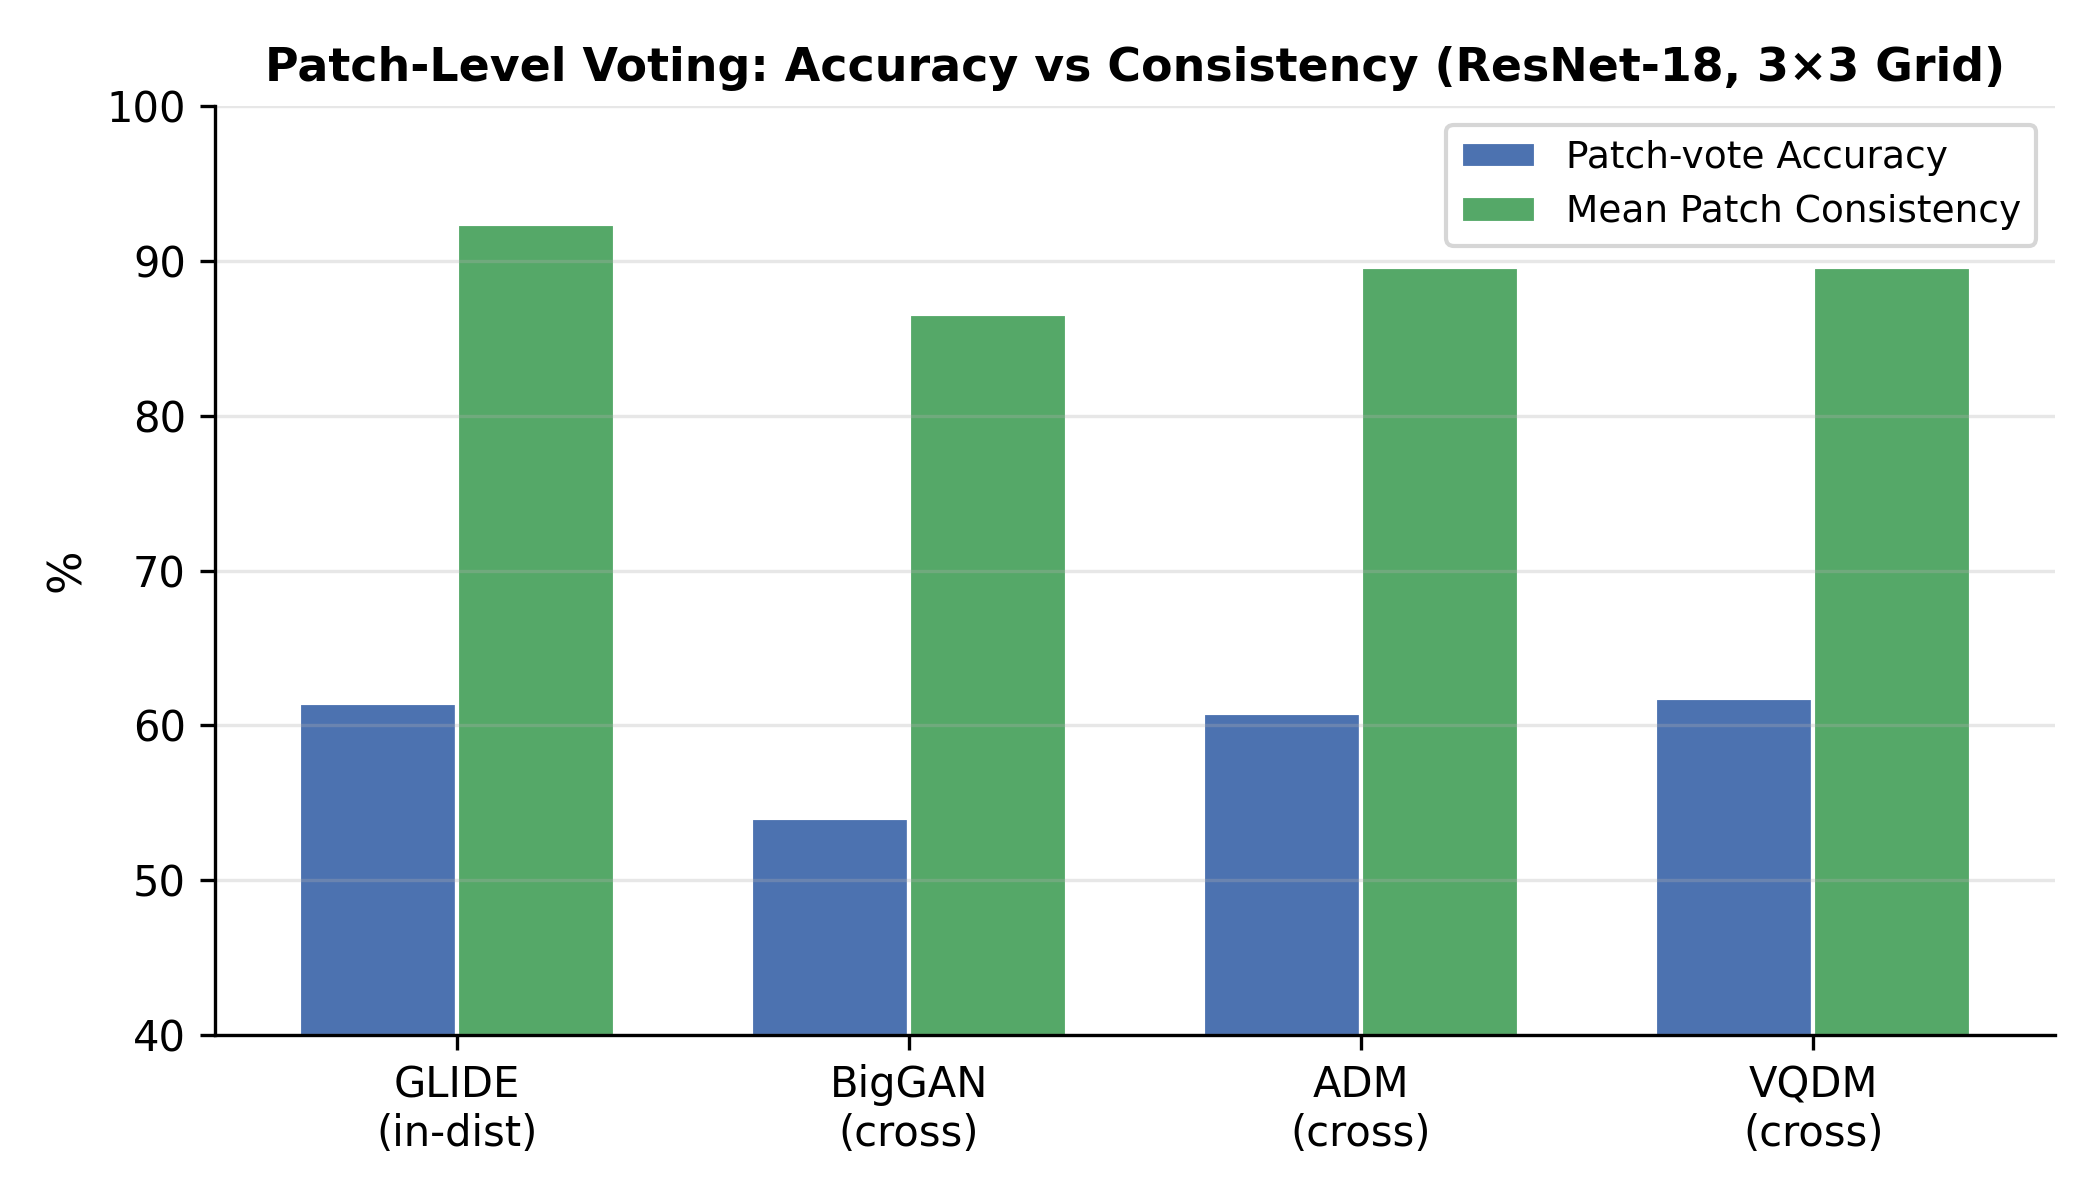
\includegraphics[width=0.75\textwidth]{fig4_patch_analysis.png}
    \caption{Patch-level majority-vote accuracy vs.\ mean patch consistency for ResNet-18 (3$\times$3 grid). High consistency despite low accuracy indicates systematic rather than localised errors.}
    \label{fig:patch}
\end{figure}


\subsection{Unsupervised Generator Clustering}

To assess whether learned features encode generator identity without explicit generator supervision, we extract features from 200 images per generator (800 total) and apply $K$-Means ($k$=4) followed by $t$-SNE visualisation.
We compare two conditions: (A) pretrained ViT-Small weights (no task adaptation), and (B) the same backbone after full fine-tuning for real-vs-fake detection.

Table~\ref{tab:cluster} and Figure~\ref{fig:cluster} report the results.
Pretrained features yield clustering Purity of 0.278 and NMI of 0.003—essentially random (chance Purity = 0.25)—confirming that off-the-shelf ViT representations do not distinguish generators.
After fine-tuning for binary detection, Purity rises to \textbf{0.559} and NMI to \textbf{0.378}: a $2\times$ improvement achieved with \emph{no explicit generator-identity supervision}.

Inspecting the cluster composition (Table~\ref{tab:cluster}), we find that the fine-tuned feature space loosely separates generator families: GLIDE images dominate one cluster, while ADM and VQDM (both latent or score-based diffusion) co-occupy two other clusters, and BigGAN is partially separated.
The $t$-SNE projection (Figure~\ref{fig:cluster}) confirms increasing inter-generator separation after fine-tuning.

\begin{table}[H]
\centering
\caption{K-Means ($k$=4) clustering quality on 800 fake images (200/generator).}
\label{tab:cluster}
\begin{tabular}{lcc}
\toprule
\textbf{Feature} & \textbf{Purity} & \textbf{NMI} \\
\midrule
Pretrained ViT-Small  & 0.278 & 0.003 \\
Fine-tuned ViT-Small  & \textbf{0.559} & \textbf{0.378} \\
\bottomrule
\end{tabular}
\end{table}

\begin{figure}[H]
    \centering
    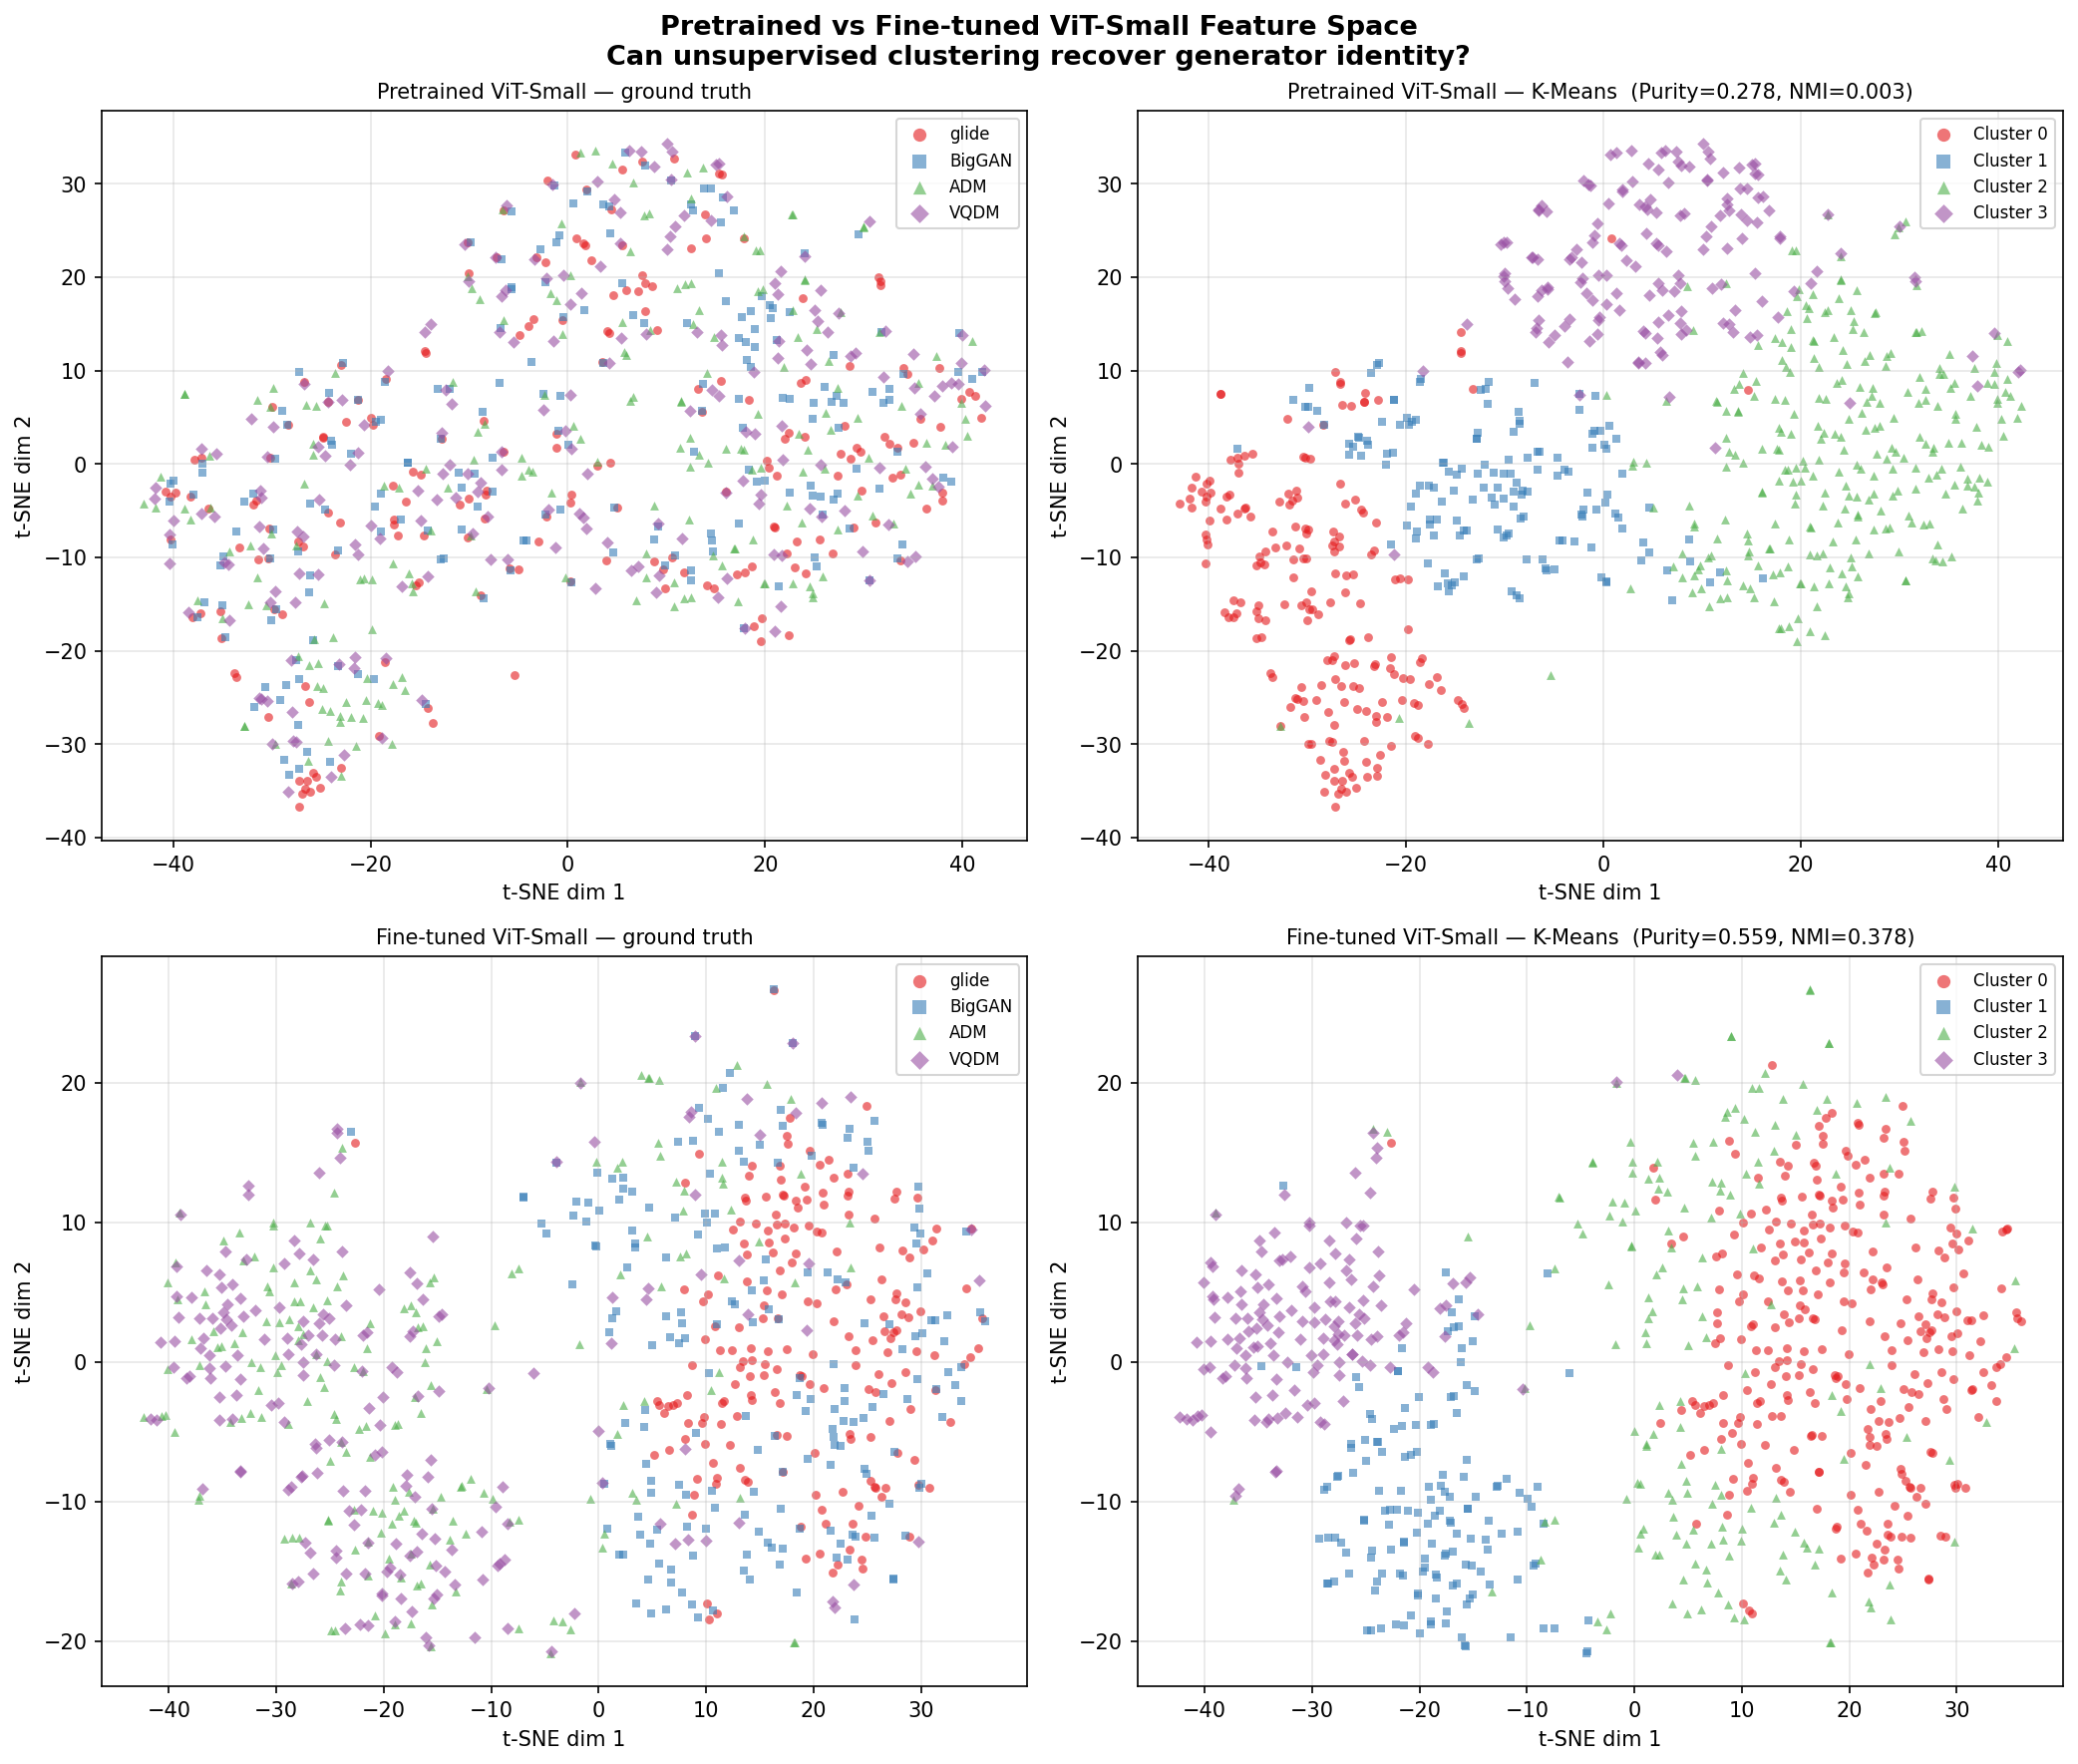
\includegraphics[width=\textwidth]{fig_cluster_compare.png}
    \caption{$t$-SNE of pretrained (top) vs.\ fine-tuned (bottom) ViT-Small features, coloured by ground-truth generator (left) and K-Means cluster (right). Fine-tuning for binary detection implicitly organises the feature space by generator family.}
    \label{fig:cluster}
\end{figure}

\section{Discussion}

\paragraph{Why do models fail on ADM and VQDM?}
Our results confirm the generalisation gap identified by Ojha~et~al.~\cite{ojha2023towards}: fine-tuned models memorise generator-specific low-level artifacts (e.g., specific noise patterns from GLIDE's denoising scheduler) that do not transfer to different diffusion architectures.
ADM uses a class-conditional score-based diffusion process, while VQDM employs vector-quantised latent diffusion—both producing artifacts in fundamentally different frequency regimes than GLIDE.

\paragraph{The promise of CLIP-based approaches.}
The superiority of CLIP-ViT KNN on hard generators (ADM, VQDM) suggests that vision-language pretraining encodes higher-level visual statistics that are more generator-agnostic.
However, its lower in-distribution accuracy (85\%) compared to fine-tuned models (98--99\%) reveals a trade-off: generality comes at the cost of in-distribution precision.

\paragraph{Towards a Mixture-of-Experts (MoE) framework.}
A natural direction for closing this gap is to combine specialised detectors with a learned routing mechanism.
We propose a three-component framework:
\begin{itemize}
    \item \textbf{GAN expert}: a fine-tuned CNN detecting frequency-domain spectral artifacts characteristic of GAN outputs.
    \item \textbf{Diffusion expert}: a reconstruction-error detector following DIRE~\cite{wang2023dire} or FIRE, specialised for diffusion-model artifacts.
    \item \textbf{Universal router}: a frozen CLIP encoder that clusters test images by visual style and routes them to the most appropriate expert.
\end{itemize}
Our unsupervised clustering experiment (Section~4.5) provides direct empirical support for this design.
Fine-tuned ViT-Small features achieve K-Means Purity of 0.559 and NMI of 0.378 with \emph{no generator-identity labels}—a $2\times$ improvement over pretrained features (Purity 0.278).
This demonstrates that detection-oriented supervision implicitly structures the feature space along generator-family boundaries, suggesting that a lightweight routing head trained on top of such features could reliably assign test images to the correct specialist expert.
If the router uses unsupervised clustering rather than a supervised generator classifier, the framework can generalise to unseen generator families—addressing the core limitation of current approaches.

\paragraph{Limitations.}
Our study uses a subset of 12\,000 training images from a single generator (GLIDE).
Results may differ with larger or more diverse training sets.
Additionally, CLIP's visual representations may themselves be biased toward certain image types seen during pretraining.


\section{Conclusion}

We conducted a systematic ablation study of AI-generated image detection across five method variants and four generators from two distinct architectural families.
Our key findings are:
(1) Full fine-tuning on a single generator achieves near-perfect in-distribution and GAN-transfer accuracy but fails on diffusion generators with different sampling mechanisms;
(2) CLIP-ViT KNN provides the best cross-generator generalisation on hard generators, supporting the value of frozen vision-language representations;
(3) Patch-level analysis reveals that detection failures are spatially uniform, pointing to global feature mismatch as the root cause;
(4) Unsupervised K-Means clustering of fine-tuned ViT-Small features achieves Purity 0.559 and NMI 0.378 with no generator-identity supervision, providing the first empirical evidence that detection-oriented training implicitly structures the feature space by generator family and validating the routing component of a future MoE framework.
These findings motivate future work on mixture-of-experts architectures that combine generator-specialised experts with a universal routing mechanism.

\section*{Acknowledgements}

The authors thank the GenImage dataset team~\cite{zhu2023genimage} and the HuggingFace community for providing accessible data mirrors.

\medskip

\bibliographystyle{plain}
\bibliography{ref}

\end{document}
